\chapter{Cronograma}
Conforme descrito na seção \ref{sec:metodology}, o trabalho foi dividido em seis etapas. Dessas etapas, apenas os modelos cujas implementações estão evidenciadas no diagrama de classes da figura \ref{fig:ClassDiagramCronograma} estão em fase de análise, os demais já concluíram essa fase. Desse modo, como entregáveis para a VF estão previstas as etapas de desenvolvimento da subseção \ref{subsec:desenvolvimento} e uma avaliação final sobre os resultados conforme a subseção \ref{subsec:avaliacao}.

\begin{figure}[!ht]
	\centering
	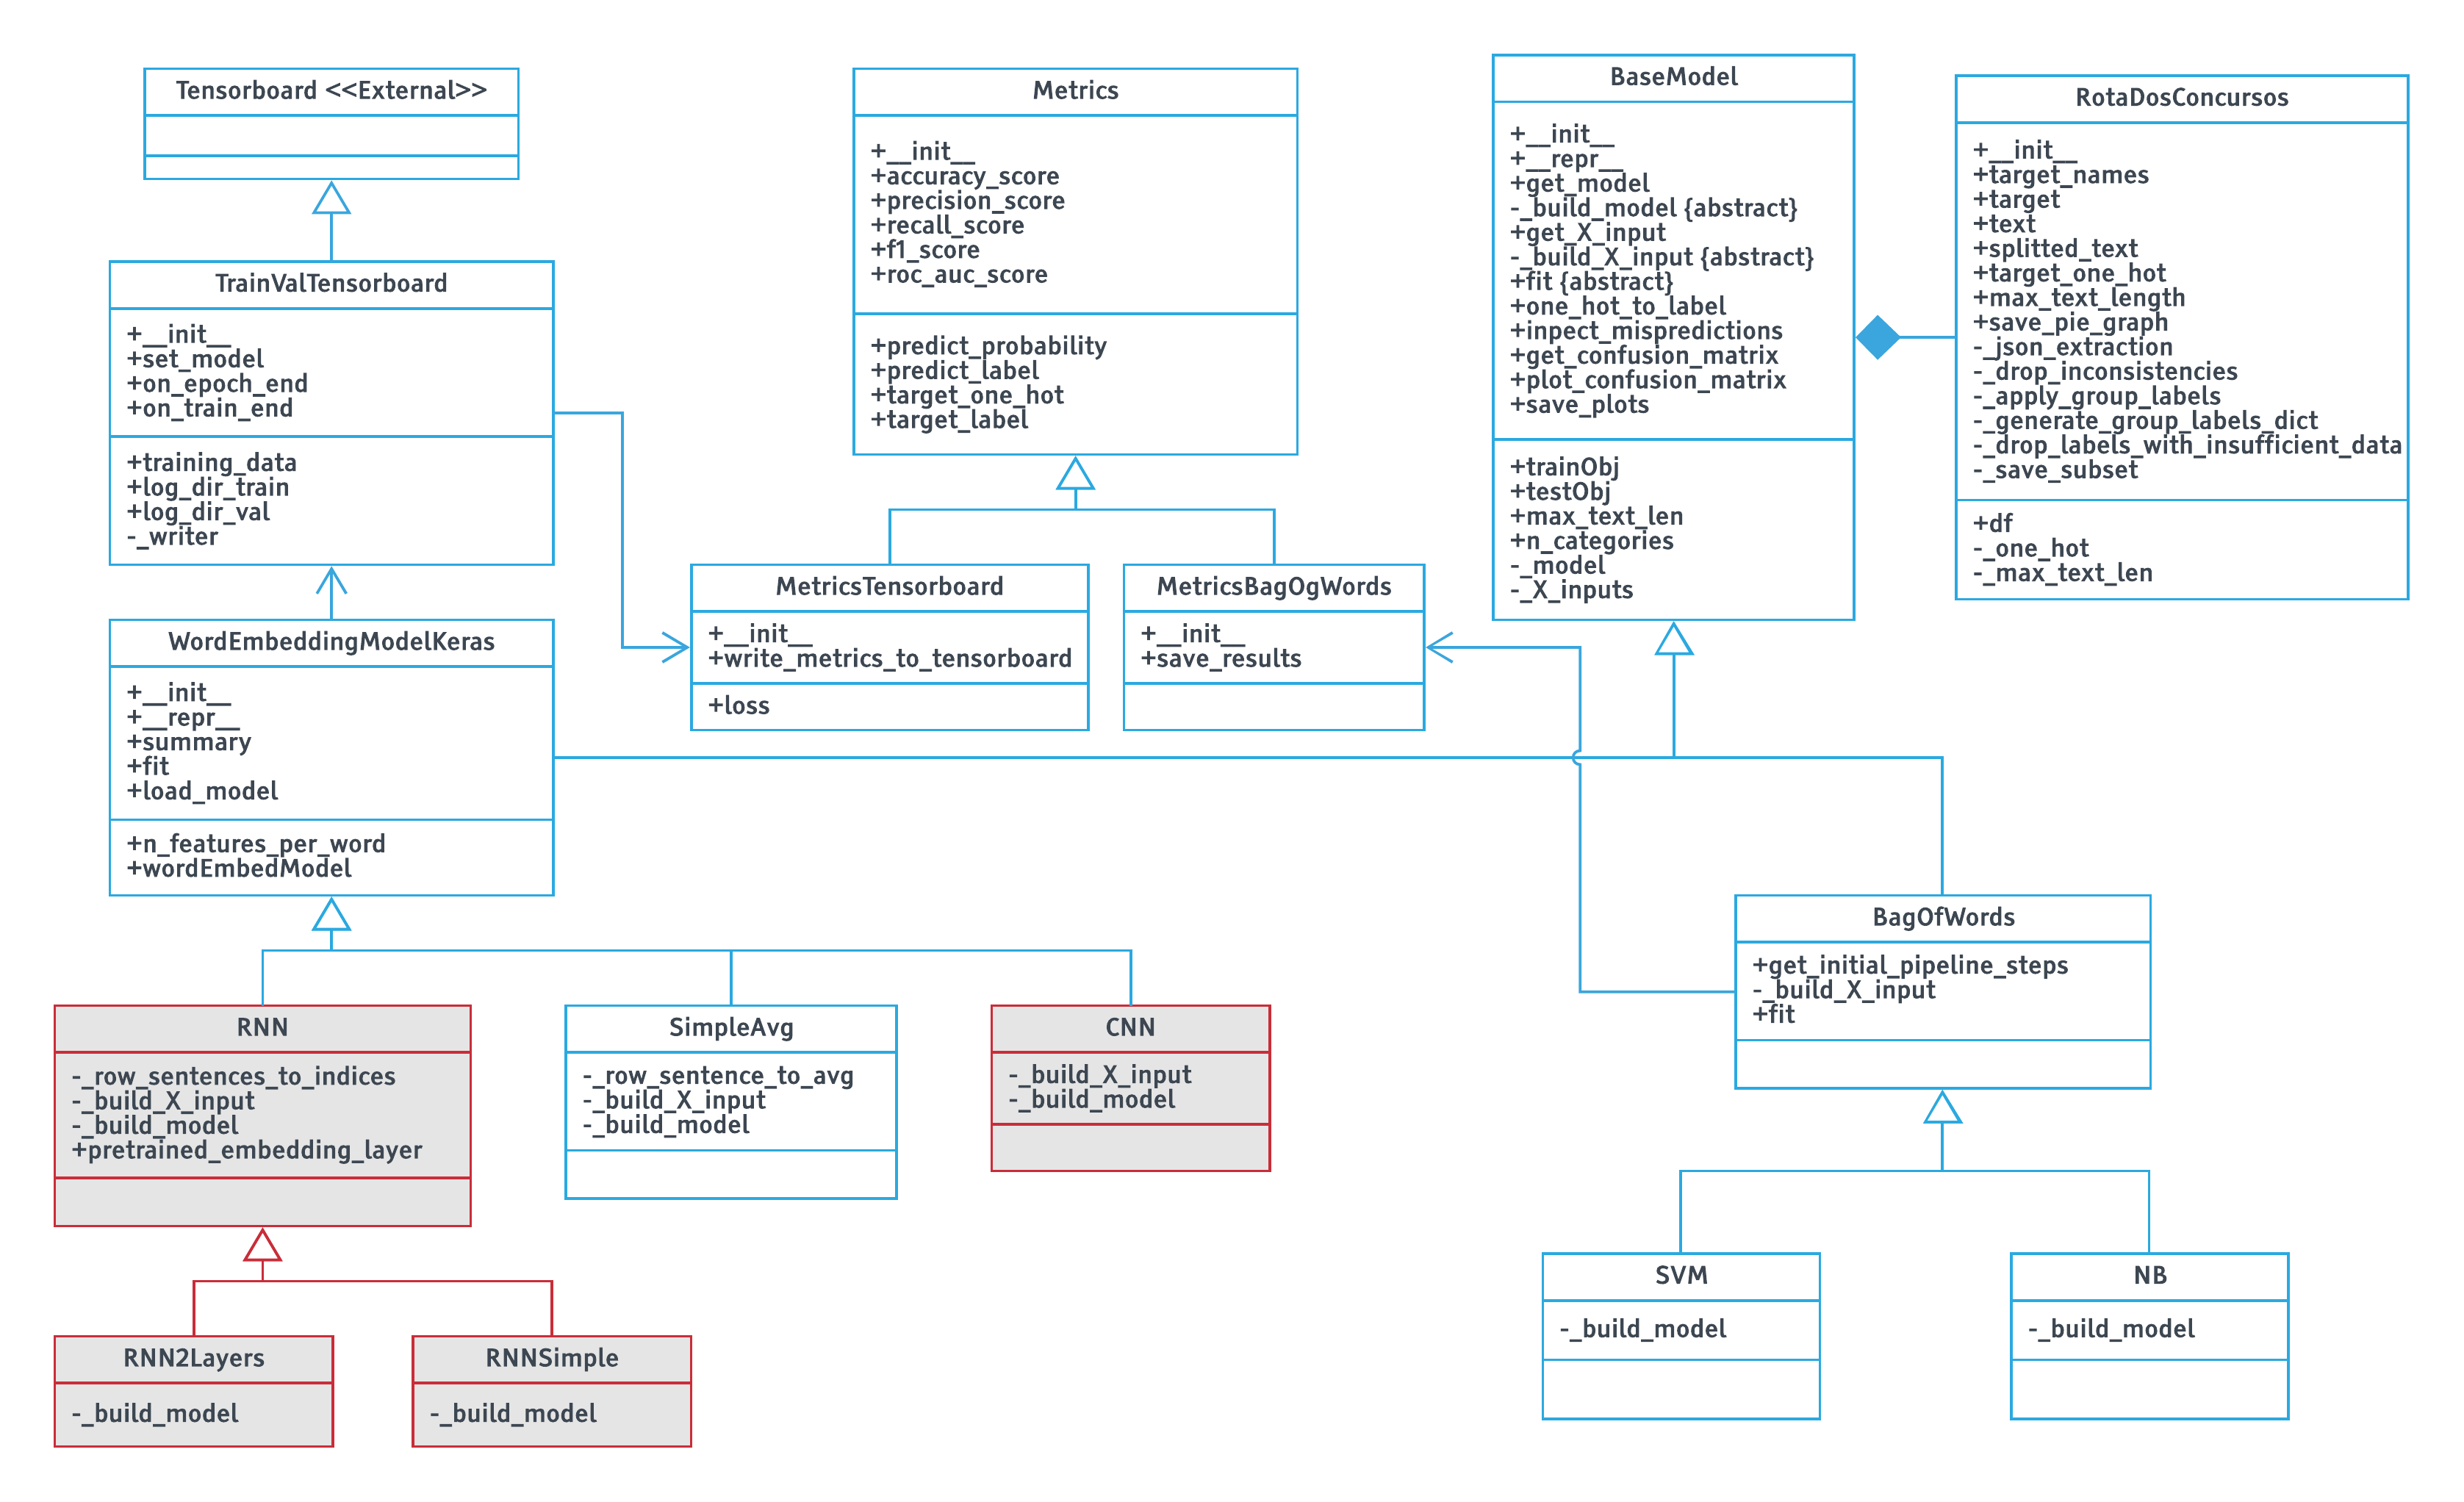
\includegraphics[width=1.16\textwidth]{figures/ClassDiagram-Cronograma.png}
	\caption{Classes em análise para a VF em destaque}
	\label{fig:ClassDiagramCronograma}
\end{figure}
